\documentclass[a4paper,12pt]{article}
\usepackage{amsmath,amssymb,amsfonts,amsthm}
\usepackage{tikz}
\usepackage [utf8x] {inputenc}
\usepackage [T2A] {fontenc} 
\usepackage[russian]{babel}
\usepackage{cmap, upgreek}
\usepackage{textcomp} 


% Так ссылки в PDF будут активны
\usepackage[unicode]{hyperref}

% вы сможете вставлять картинки командой \includegraphics[width=0.7\textwidth]{ИМЯ ФАЙЛА}
% получается подключать, как минимум, файлы .pdf, .jpg, .png.
\usepackage{graphicx}
% Если вы хотите явно указать поля:
\usepackage[margin=1in]{geometry}
% Или если вы хотите задать поля менее явно (чем больше DIV, тем больше места под текст):
% \usepackage[DIV=100]{typearea}

\usepackage{fancyhdr}

\newcommand{\bbR}{\mathbb R}%теперь вместо длинной команды \mathbb R (множество вещественных чисел) можно писать короткую запись \bbR. Вместо \bbR вы можете вписать любую строчку букв, которая начинается с '\'.
\newcommand{\eps}{\varepsilon}
\newcommand{\bbN}{\mathbb N}
\newcommand{\dif}{\mathrm{d}}

\newtheorem{Def}{Определение}


\pagestyle{fancy}
\makeatletter % сделать "@" "буквой", а не "спецсимволом" - можно использовать "служебные" команды, содержащие @ в названии
\fancyhead[L]{\footnotesize Электричество и магнетизм}%Это будет написано вверху страницы слева
\fancyhead[R]{\footnotesize ФМХФ МФТИ}
\fancyfoot[L]{\footnotesize \@author}%имя автора будет написано внизу страницы слева
\fancyfoot[R]{\thepage}%номер страницы —- внизу справа
\fancyfoot[C]{}%по центру внизу страницы пусто

\renewcommand{\maketitle}{%
	\noindent{\bfseries\scshape\large\@title\ \mdseries\upshape}\par
	\noindent {\large\itshape\@author}
	\vskip 2ex}
\makeatother
\def\dd#1#2{\frac{\partial#1}{\partial#2}}


\title{3.2.6 \\ Исследование гальванометра}
\author{Егор Берсенев} 
\date{15 апреля 2016 г.}

\begin{document}
	\maketitle
	\section{Цель работы}
		 Изучение работы высокочувствительного зеркального гальванометра магнитоэлектрической системы в режимах измерения постоянного тока и электрического заряда.
	\section{Оборудование}
		Зеркальный гальванометр с осветителем и шкалой, источник постоянного напряжения, делитель напряжения, магазин сопротивлений, эталонный конденсатор, вольтметр, переключатель, ключи, линейка.
	\section{Теоретическая часть}
		Уравнение движения рамки сопротивлением $R$, площадью $S$ с $N$ витками, по которым течет ток $I$ в постоянном магнитном поле $B$ имеет вид:
		\begin{equation}
			J\ddot{\varphi}+\frac{\left(BSN\right)^2}{R_\upvarsigma}\dot{\varphi} + D\varphi = BSNI \end{equation}\begin{equation}
			\ddot{\varphi} +2\gamma\dot{\varphi}+\omega_0^2\varphi = KI
		\end{equation}
		\subsection{Режим измерения постоянного тока}
		Считаем колебания затухшими, т.е. $\ddot{\varphi} = \dot{\varphi} = 0$, когда 
		\begin{equation}
			\varphi = \frac{K}{w_0^2}I = \frac{BSN}{D}I = \frac{I}{C_1}
		\end{equation}, 
		где $C_1 = \cfrac{D}{BSN}$ --- динамическая постоянная гальванометра.
		
		\subsection{Свободные колебания рамки}
		Пусть $I = 0$ и выполнены следующие начальные условия: $t = 0, \varphi = 0, \dot{\varphi} = \dot{\varphi}_0$. Тогда уравнение движения примет вид:\begin{equation}
			\ddot{\varphi} +2\gamma\dot{\varphi}+\omega_0^2\varphi = 0
		\end{equation}
		Рассмотрим три варианта движения рамки:
		\paragraph{Колебательный режим}
		
		В колебательном режиме $\gamma \le \omega_0$. Теперь пусть $\omega^2 = \omega_0^2 - \gamma^2$ В этом случае решение уравнения имеет вид:
		\begin{equation}
			\varphi = \frac{\dot{\varphi}_0}{\omega_0}e^{-\gamma t}\sin\omega t
		\end{equation}
		В этом случае период колебаний равен $T = \cfrac{2\pi}{\sqrt{w_0^2-\gamma^2}}$
		
		\paragraph{Критический режим}
		
		В критическом режиме $\gamma =  \omega_0$. В этом случае движение не имеет колебательного характера, и уравнение движения имеет вид:
		\begin{equation}
			\varphi = \dot{\varphi}_0te^{-\gamma t}
		\end{equation}
		
		\paragraph{Затухание велико}
		
		В этом режиме $\gamma \ge \omega_0$. Это случай переуспокоенного гальванометра.Теперь пусть $\varkappa^2 = \gamma^2 - \omega_0^2$. Уравнение движения имеет вид:
		\begin{equation}
		\varphi = \frac{\dot{\varphi}_0}{\omega_0}e^{-\gamma t}\sinh\varkappa t
		\end{equation}
		В этом случае движение все еще апериодическое, но система приближается к равновесию медленнее, чем в критическом режиме.
		
		\subsection{Режим измерения заряда}
		Период свободных колебаний гальванометра оказывается очень большим. Если через рамку пропустить короткий импульс тока, то можно считать, что весь ток успевает пройти при неотклоненном положении рамки. В этом случае уравнение движения сводится к следующему:
		\begin{equation}
		\dot{\varphi}(\tau) = Kq
		\end{equation}
		
		Максимальный отброс достигается при \begin{equation}
			\varphi_{max} =  =\frac{ \dot{\varphi}(\tau)}{\omega_0} = \frac{Kq}{\omega_0}
		\end{equation}
		\subsection{Определение динамической постоянной}
		Соберем схему по рисунку:
		\newline
		
		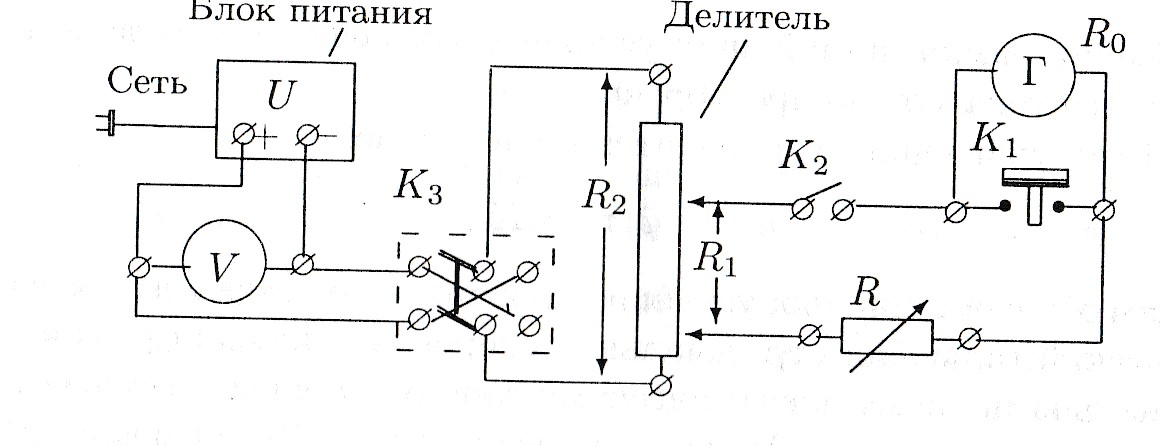
\includegraphics[width = 0.7\linewidth]{pic1}
		
		
		При малых $R$ сила тока, протекающего через гальванометр может быть вычислена по формуле:
		\begin{equation}
		I = U_0 \frac{R_1}{R_2}\frac{1}{R+R_0}
		\end{equation}
		Угол отклонения рамки связан с координатой зайчика следующим образом: $x = a\tan(2\varphi)$ При малых углах можно считать, что $\varphi = \frac{x}{2a}$. Динамическую постоянную 
		\begin{equation}
			C_1 = \frac{I}{\varphi} = \frac{2aI}{x}
		\end{equation}
		как правило выражают в единицах$ \left[\frac{\text{А}}{\text{мм} / \text{м}}\right]$
		\subsection{Определение критического сопротивления гальванометра}
		Скорость затухания характеризуется логарифмическим декрементом затухания:
		\begin{equation}
			\theta  = \ln\frac{x_n}{x_{n+1}} = \gamma T = \frac{2\pi R_3}{\sqrt{\left(R_0+R\right)^2-R_3^2}},
		\end{equation} 
		где $R_3 = R_0 + R_{cr}$.
		
		Отсюда получаем:
		\begin{equation}
		R_{cr} = \frac{1}{2\pi}\sqrt{\frac{\Delta X}{\Delta Y}}-R_0
		\end{equation}
	\subsection{Определение баллистической постоянной}
	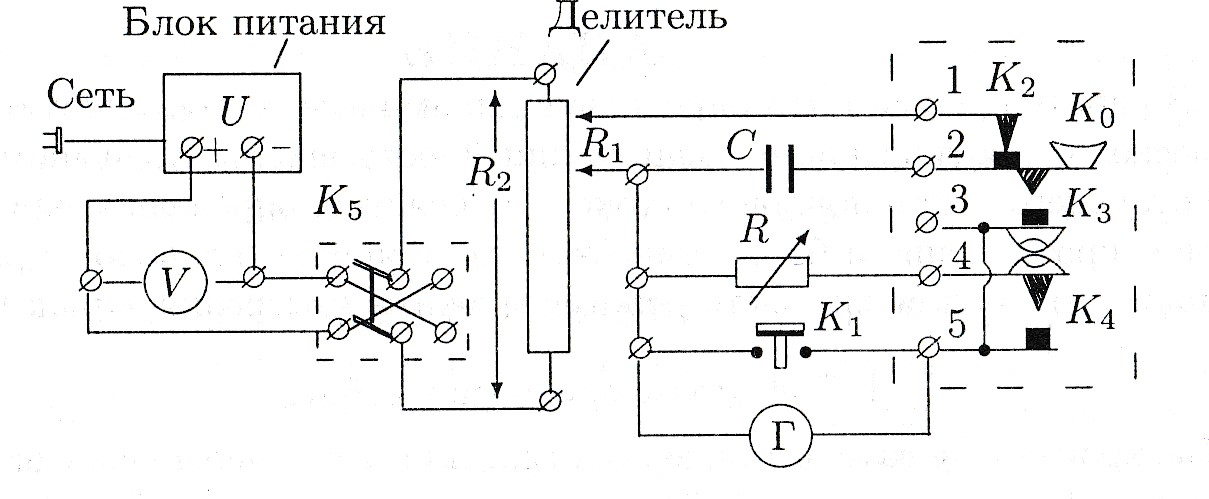
\includegraphics[width = 0.7\linewidth]{pic2}
	
	Конденсатор заряжается до напряжения $U_c = \frac{R_1}{R_2}U_0$, при этом его заряд равен $q = CU_c = \frac{R_1}{R_2}U_0C$.
	
	Баллистическая постоянная определяется при критическом сопротивлении:
\begin{equation}
	C_{q{cr}} = \frac{q}{\varphi_{max}} = 2a\frac{R_1}{R_2}\frac{U_0 C}{I_{max}}
\end{equation}

\section{Ход работы}
\subsection{Определение динамической постоянной}
Соберем схему 1 и снимем зависимость отклонения зайчика от сопротивления магазина при постоянном положении делителя $\frac{R_1}{R_2} = \frac{1}{2000}$.

Построим таблицу результатов:
\begin{table}[h]
	\caption{Определение динамической постоянной}
	\label{my-label}
	\begin{tabular}{|l|l|l|l|l|l|l|l|l|l|l|}
		\hline
		$R$     & 0.9    & 1.4       & 2.4    & 2.9    & 3.4    & 3.9      & 4.9    & 5.4    & 5.9   & 6.4     \\ \hline
		
		$x_+$   & 23.1   & 174     & 11.6   & 10     & 8.7    & 7.6         & 6.3    & 5.8    & 5.3   & 4.9     \\ \hline
		$x_-$   & 23.9   & 18       & 11.9   & 10.2   & 8.9    & 7.9       & 6.5    & 6      & 5.5   & 5.1     \\ \hline
		$x_{av}$& 23.5   & 17.7     & 11.75  & 10.1   & 8.8    & 7.75      & 6.4    & 5.9    & 5.4   & 5     \\ \hline
		$I$     & 456.95 & 343.28 & 229.24 & 195.58 & 172.07 & 152.99  & 125.23 & 114.81 & 105.99 & 98.43   \\ \hline
	\end{tabular}
\end{table}

\newpage
	Построим график:
	
	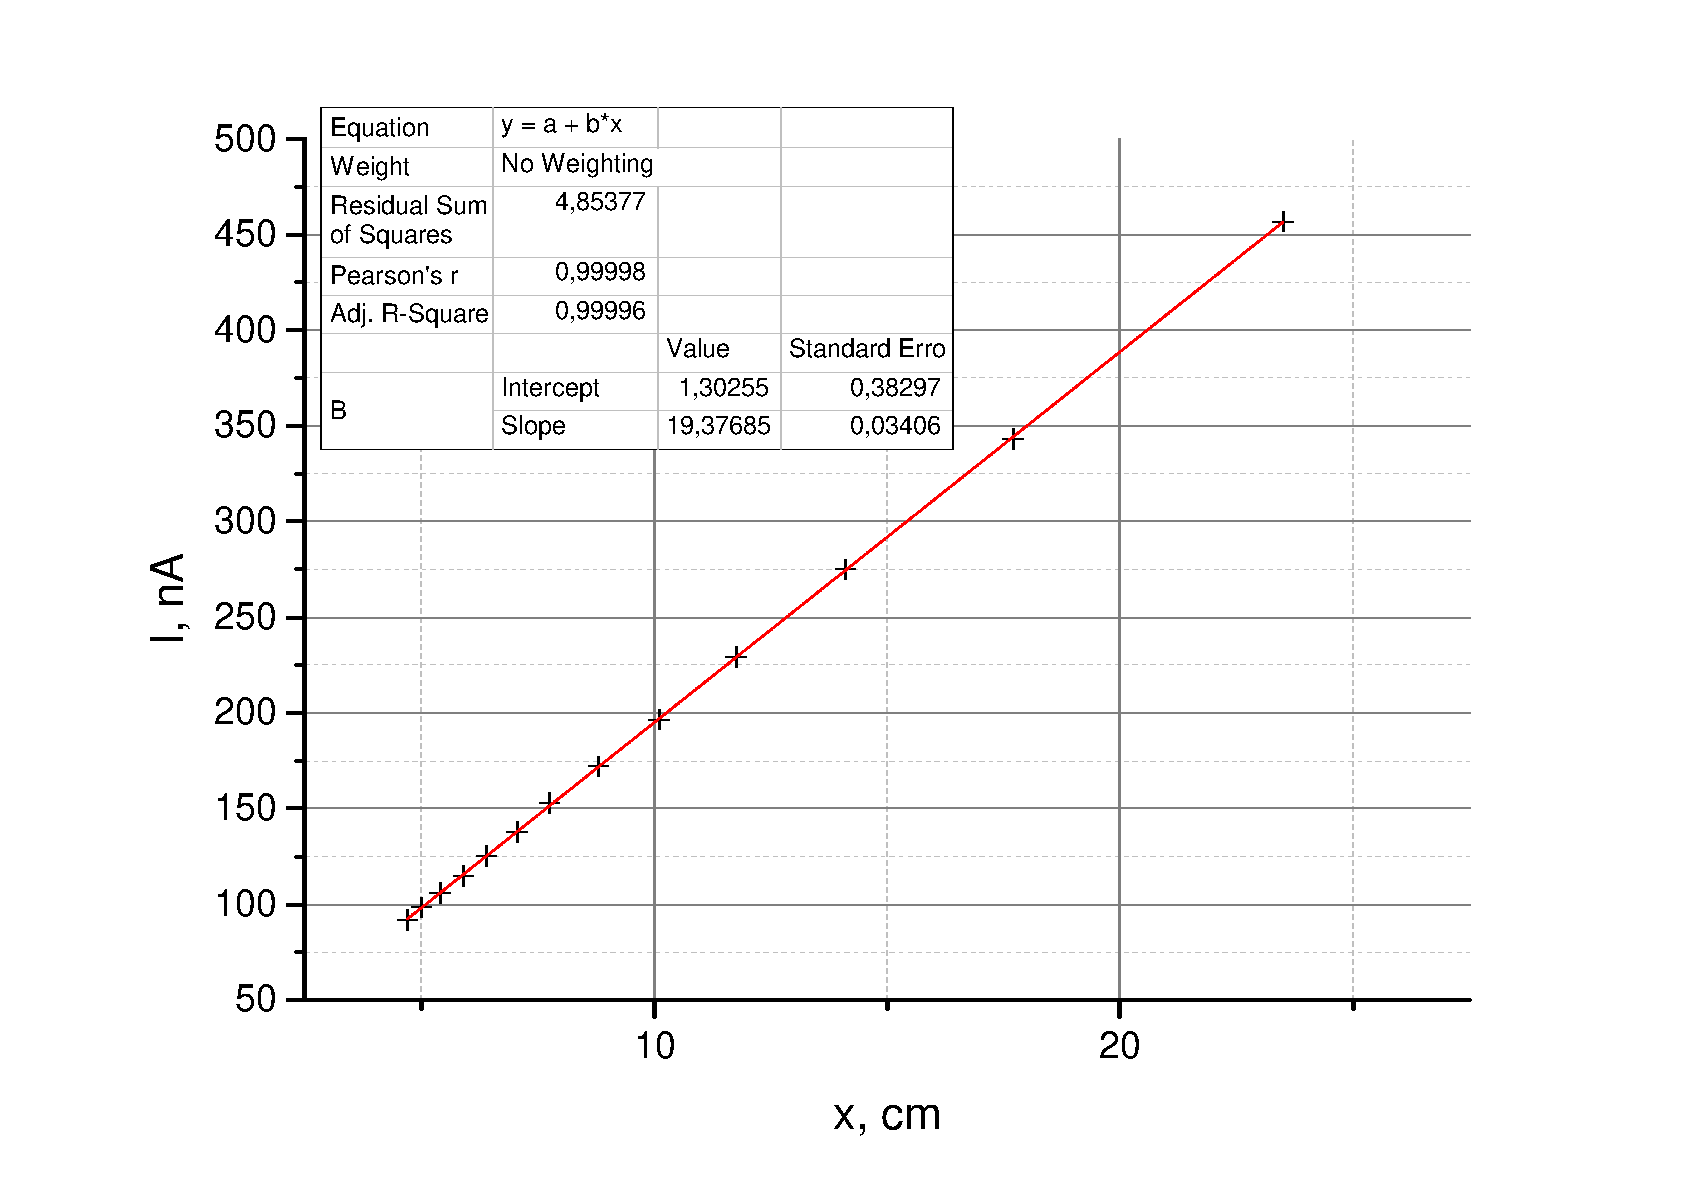
\includegraphics[width = 0.7\linewidth]{graph1}
	
	
\subsection{Определение критического сопротивления}
Пронаблюдаем свободные колебания рамки. Измерим два последовательных отклонения и рассчитаем логарифмический декремент затухания.

\begin{table}[h]
	\centering
	\caption{Логарифмический декремент затухания}
	\label{my-label}
	\begin{tabular}{|l|l|l|l|l|l|l|}
		\hline
		$x_n$ & 20.2  & 17.9  & 16    & 14.7  & 12.7  & 17.2  \\ \hline
		$x_{n+1}$ & 17.9  & 16    & 14.7  & 12.7  & 11.4  & 15.3  \\ \hline
		$\theta $ & 0.121 & 0.112 & 0.085 & 0.146 & 0.108 & 0.117 \\ \hline
	\end{tabular}
\end{table}

Отсюда получаем: $\bar{\theta} = 0.115 \pm 0.005$

Измерим также период свободных колебаний рамки: $T = 2.5\,$c

Подберем наибольшее сопротивление магазина, при котором зайчик не проходит через нулевое положение. Это сопротивление $R = 4.5\,$кОм. Проведем измерения 

\begin{table}[h!]
	\centering
	\caption{Измерение логарифмического декремента}
	\label{my-label}
	\begin{tabular}{|l|l|l|l|l|l|}
		\hline
		$R$, кОм & $\left(R+R_0\right)^2$, кОМ    & $x_n$, см     & $x_{n+1}$, см      &  $\theta$ & $\frac{1}{\theta^2}$    \\ \hline
		13.5  & 199.09  & 2.3 & 0.3 & 2.037 & 0.241 \\ \hline
		15.75 & 267.65  & 2.8 & 0.5 & 1.723 & 0.337 \\ \hline
		18    & 346.33  & 6.7 & 1.2 & 1.720 & 0.338 \\ \hline
		20.25 & 435.14  & 3.3 & 0.8 & 1.417 & 0.498 \\ \hline
		22.5  & 534.07  & 3.4 & 0.9 & 1.329 & 0.566 \\ \hline
		24.75 & 643.13  & 6.2 & 1.7 & 1.294 & 0.597 \\ \hline
		27    & 762.31  & 5.9 & 1.8 & 1.187 & 0.710 \\ \hline
		29.25 & 891.62  & 5.7 & 1.9 & 1.099 & 0.829 \\ \hline
		31.5  & 1031.05 & 5.4 & 1.9 & 1.045 & 0.917 \\ \hline
		36    & 1340.29 & 5   & 2   & 0.916 & 1.191 \\ \hline
		40.5  & 1690.03 & 4.7 & 2.1 & 0.806 & 1.541 \\ \hline
	\end{tabular}
\end{table}
\pagebreak
Построим график:

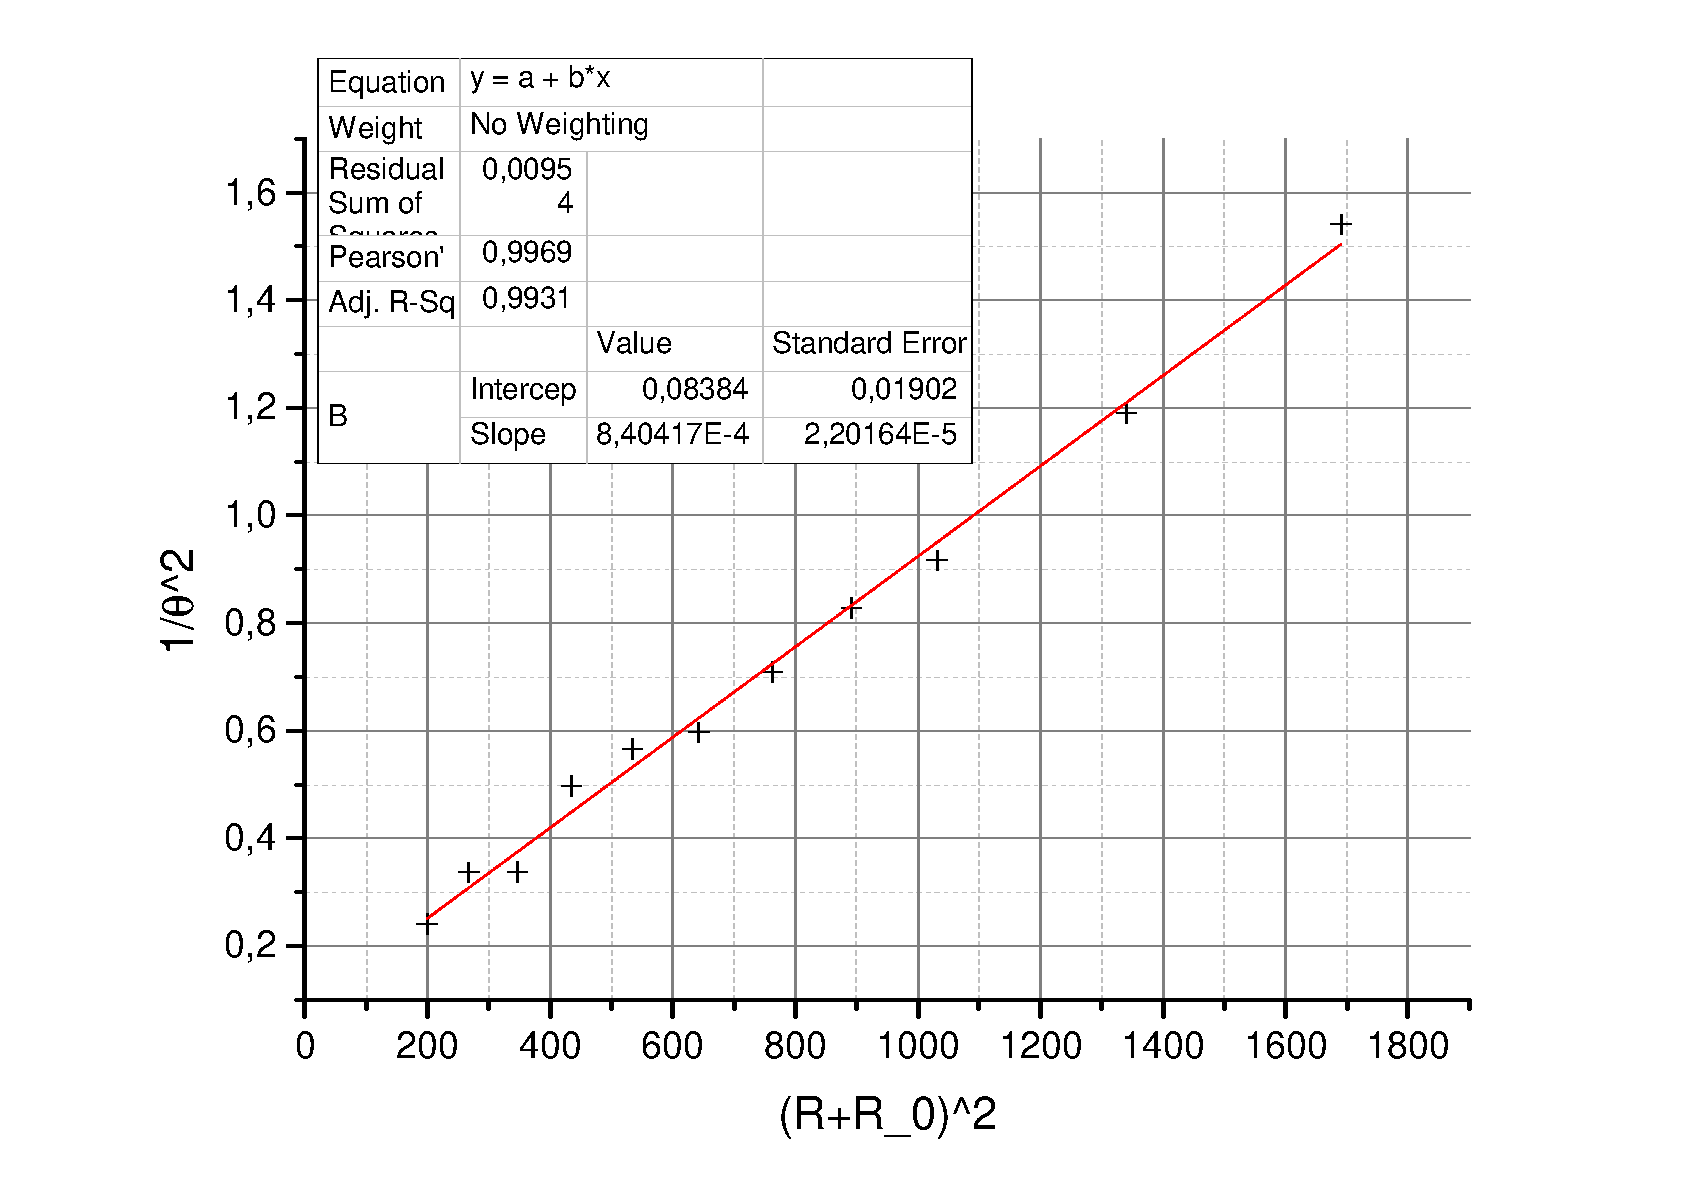
\includegraphics[width = 0.7\linewidth]{graph2}

Критическое сопротивление: $R_{cr} = 4.88\pm 0.43$ кОм.
\subsection{Баллистический режим}
	Соберем схему по рисунку: 
	\newline
	
	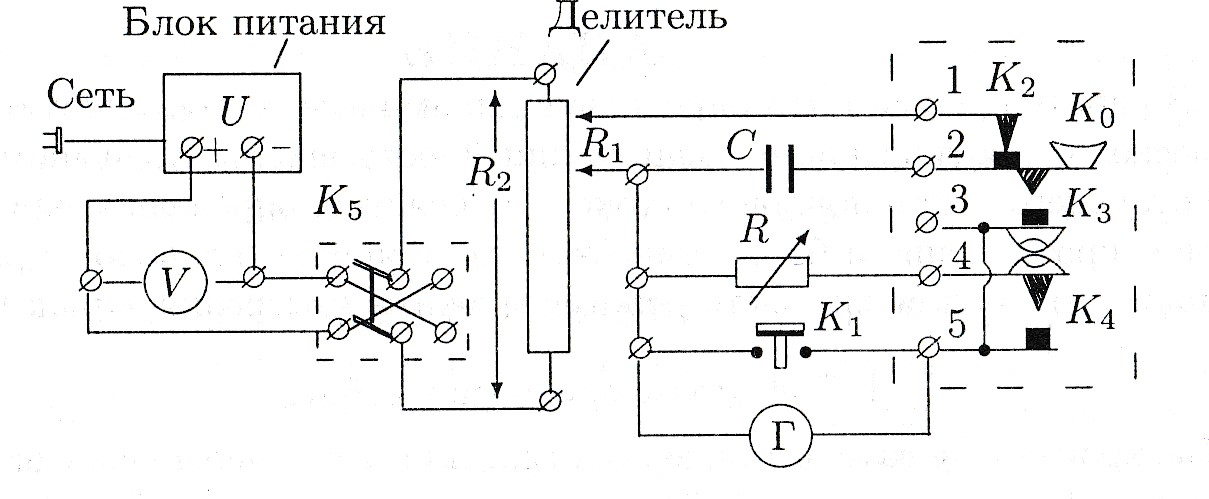
\includegraphics[width = 0.9\linewidth]{pic2}
	
	Измерим первый отброс в свободном режиме при положении делителя $\cfrac{R_1}{R_2} = \cfrac{1}{15}$
	

	
	\begin{table}[h]
		\begin{tabular}{|l|l|l|l|l|l|l|l|l|l|}
			\hline
			$R$, кОм& 50    & 40    & 25    & 15    & 10    & 5      & 4.5    & 4      & 3.5    \\ \hline
			$\left(R+R_0\right)^{-1}\cdot 10^3$, кОм$^{-1}$& 19.76 & 24.62 & 39.05 & 64.06 & 94.25 & 178.25 & 195.69 & 216.92 & 243.31 \\ \hline
			$ x_{max}$, см & 17.2  & 16.5  & 14.7  & 12.1  & 11.3  & 7.6    & 7.3    & 6.6    & 6      \\ \hline
		\end{tabular}
	\end{table}
	
	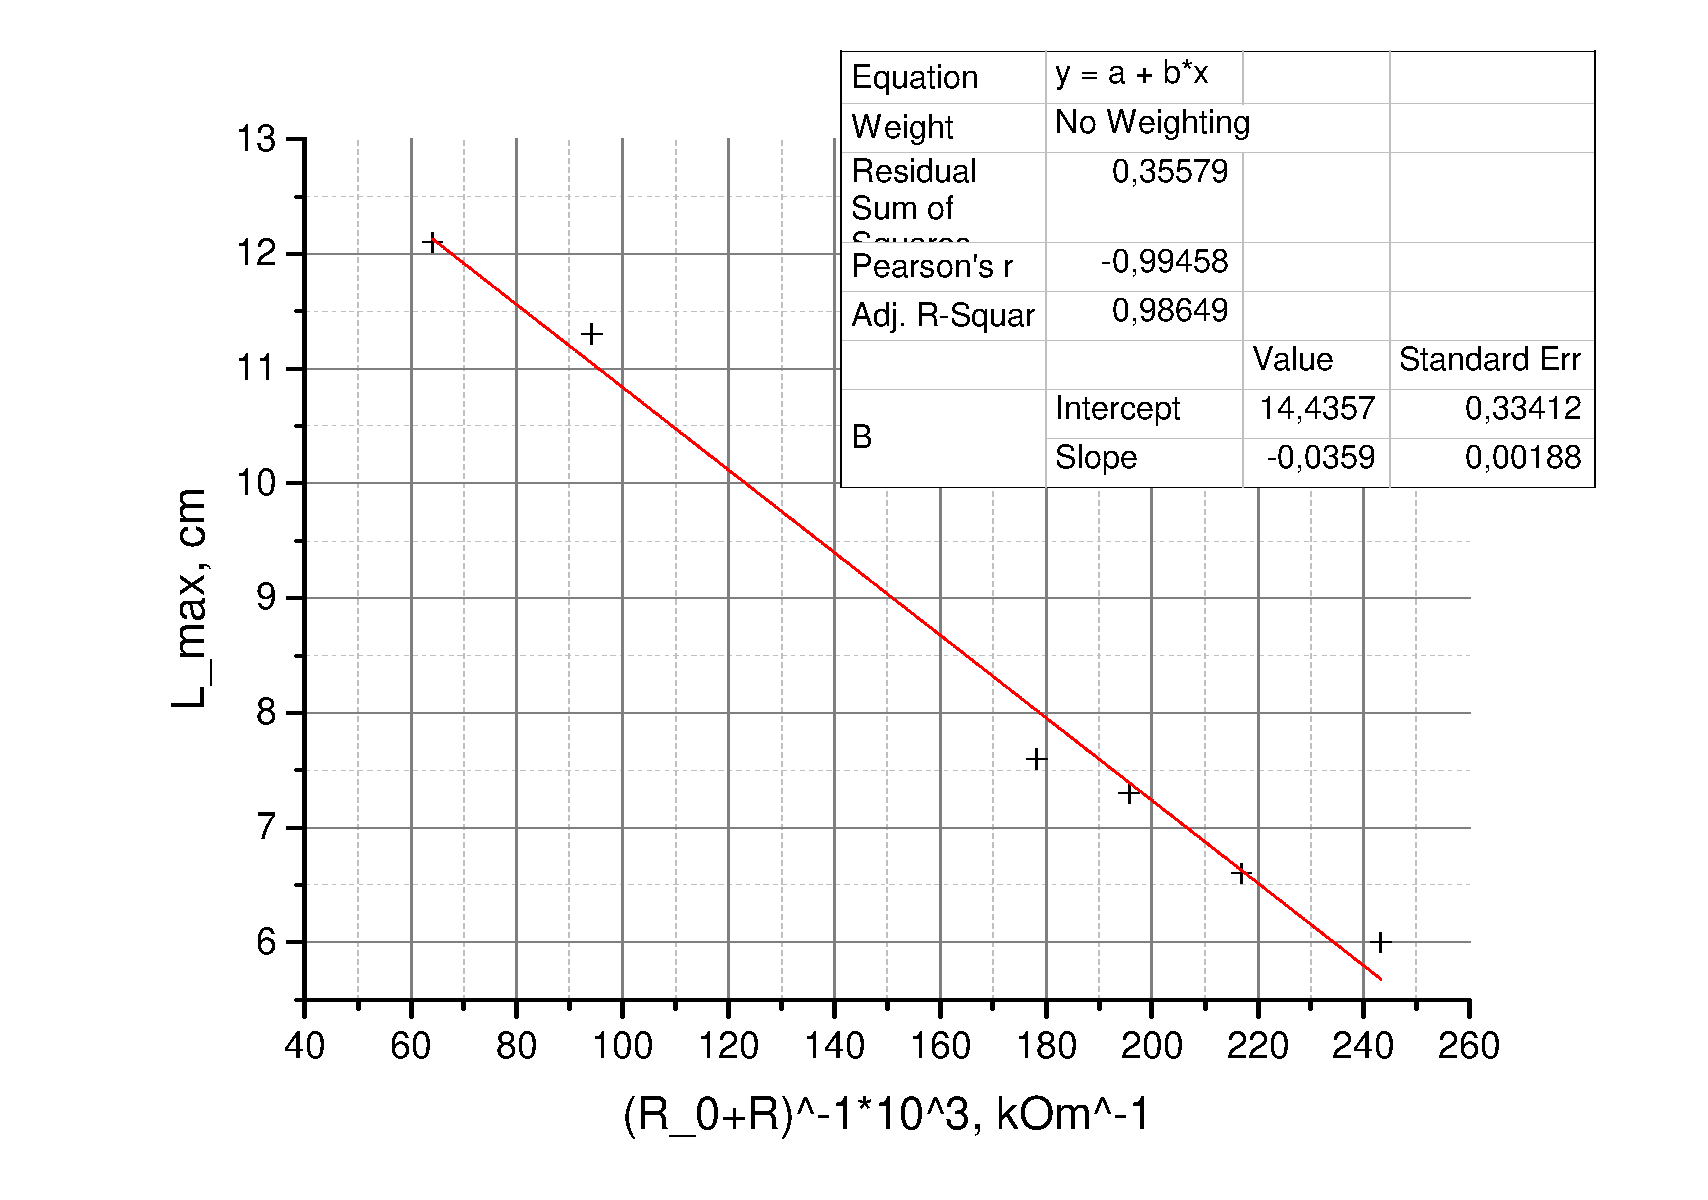
\includegraphics[width = 0.7\linewidth]{graph3}


	Критическое сопротивление : $4.71\pm 0.47$ кОм.




Рассчитаем баллистическую постоянную в критическом режиме: $$C_{q_{cr}} = 2a\frac{R_1}{R_2}\frac{U_0C}{I_{max}} = 6.76\cdot10^{-10}\,\frac{\text{К}}{\text{мм/м}}$$

Время релаксации $t = R_0C = 610\cdot2\cdot10^{-6}=1.22\cdot10^{-3}\ll T  = 2.5$ с. 
	\section{Вывод}
		Критическое сопротивление, измеренное тремя путями сошлось в пределах погрешности, что позволяет говорить о точном измерении. Время релаксации много меньше периода свободных колебаний, что подтверждает наше предположение о том, что можно пренебречь начальным углом и угловой скоростью.

		
\end{document}


